\chapter{Simulazioni di immagini lensate}
\label{cap:simulazioni}
Nei capitoli precedenti si è cercato di capire come inferire la presenza di una sotto-struttura di materia oscura a partire dai dati astronomici, ovvero dalle osservabili legate allo strong gravitational lensing. Tuttavia, data la complessità del problema, è fondamentale comprendere come variazioni della lente, della sorgente e della configurazione geometrica del sistema si manifestino singolarmente nelle immagini osservative.

A questo scopo, nel presente capitolo vengono mostrate simulazioni in cui diversi parametri sono variati in maniera controllata, analizzando dapprima un caso di riferimento privo di perturbazioni. Successivamente, viene introdotto un perturbatore modellato mediante due profili differenti, quello isotermo ellittico e quello di Navarro, Frenk e White (NFW, Eq. \ref{eq:NFW}).

In apertura si presenta brevemente il software utilizzato, introducendo la libreria \texttt{PyLensLib} e descrivendo sinteticamente l'architettura del codice sviluppato.

\section{Il software utilizzato}
Le simulazioni presentate nel seguito sono state realizzate mediante la libreria \texttt{PyLensLib}, sviluppata da Massimo Meneghetti. Essa permette di implementare le principali relazioni teoriche utilizzate nel lensing gravitazionale forte e introdotte nei Capitoli precedenti, secondo il formalismo comunemente adottato in letteratura \parencite{Meneghetti2022}. In questa sezione ne vengono richiamate brevemente le funzionalità rilevanti e le relative applicazioni al codice sviluppato per il presente lavoro. Successivamente si riporta schematicamente la struttura del codice e i parametri di base attribuiti alle diverse funzioni presenti. Ove non diversamente specificato, tali parametri sono da intendersi come costanti per tutta la struttura del codice.
\newpage

\subsection{Introduzione a \texttt{PyLensLib}}
La libreria scientifica \texttt{PyLensLib}, sviluppata in linguaggio di programmazione \texttt{Python}, è un software open-source che nasce per simulare sistemi di lenti gravitazionali dalle scale del microlensing fino agli ammassi di galassie \parencite{PyLensLib}. In particolare, il pacchetto si concentra su simulazioni astrofisiche nell'ambito di lensing gravitazionale forte ad opera di galassie su galassie ed ammassi.

La classe base utilizzata per simulare una lente è \texttt{genlen}, che gestisce la creazione della griglia, la ricerca delle linee critiche ed il calcolo delle corrispondenti caustiche. Vi sono poi otto classi figlie, che ne ereditano le caratteristiche implementando ciascuna un profilo analitico differente; quelle rilevanti ai fini delle successive simulazioni sono \texttt{sie} per il profilo SIE, \texttt{nfwell} per il profilo di Navarro, Frenk e White e \texttt{compositeModel}, usato per combinare più profili analitici fra loro e introdurre eventuali perturbatori.

La classe base per modellare la sorgente, invece, è \texttt{gensrc}. Da essa ereditano altre sette classi; l'unica fra queste utilizzata successivamente nel codice è \texttt{sersic}, la quale implementa la brillanza superficiale di una sorgente estesa seguendo il profilo di Sérsic (Eq. \ref{eq:Sersic}).

La generazione delle immagini viene gestita internamente dalla libreria tramite \emph{ray tracing}.
Quando viene definito l'oggetto lente mediante il relativo profilo di densità, è calcolato internamente il campo di deflessione associato $\alpha(\theta)$ su tutta la griglia numerica. Successivamente, durante la costruzione dell'oggetto sorgente, il campo di deflessione della lente passata in input viene utilizzato per applicare puntualmente l'equazione della lente (Eq. \ref{eq:lens_eq_real}) a ciascun punto $\theta$ del piano immagine, ricavando la corrispondente posizione $\beta(\theta)$ sul piano della sorgente. Poiché la distribuzione di brillanza superficiale della sorgente è nota a priori, ad ogni pixel dell'immagine viene assegnato il valore di brillanza associato al punto $\beta$ corrispondente, ottenendo così l'immagine lensata finale.

La libreria include anche strumenti per la simulazione degli effetti osservativi, come ad esempio il rumore strumentale, nonché moduli dedicati alla costruzione di scenari cosmologici più realistici. Tali funzionalità permettono di includere nel modello alcune delle complessità discusse nel Capitolo \ref{cap:SGL+DM}; tuttavia, esse non sono state utilizzate nel presente lavoro, in quanto l'obiettivo è limitato all'analisi delle deformazioni indotte dal lensing in condizioni ideali e controllate.

\subsection{Architettura del codice}
Il codice utilizzato per sviluppare le simulazioni e le relative immagini è stato scritto in linguaggio \texttt{Python}, con l'ausilio della libreria appena introdotta, ovvero \texttt{PyLensLib}, ma anche di \texttt{numpy}, libreria specifica per la programmazione numerica, e \texttt{astropy}, un insieme di pacchetti pensati appositamente per l'utilizzo in contesti astronomici. Come ausilio per la visualizzazione grafica si è utilizzata la libreria \texttt{matplotlib}; tramite \texttt{pathlib}, invece, si è creata una cartella specifica per raccogliere gli output del codice, chiamata \texttt{outputs}.

La cosmologia di riferimento è stata definita tramite il metodo \texttt{FlatLambdaCDM()} di \texttt{astropy}, che accetta come parametri la costante di Hubble al tempo presente, posta a \texttt{H0 = 70.0}, e la densità di materia al tempo presente, posta a \texttt{Om0 = 0.3}, coerentemente con quanto era stato riportato in Tabella \ref{tab:density_parameters_LCDM}.

La griglia delle immagini è stata definita una volta sola all'inizio per coerenza delle rappresentazioni e delle simulazioni, scegliendo un campo visivo di $6.0"$. Nel seguito, esso è visualizzato tramite pannelli quadrati di lato pari a 220 pixel; l'angolo $\theta$ sul piano dell'immagine è stato definito dividendo il campo visivo per il numero di pixel e centrandolo rispetto all'origine. In questo frangente si sono definiti anche il redshift della lente, pari a $z_l=0.5$, e quello della sorgente, pari a $z_s = 2.0$, mantenuti costanti nel resto del codice. Tali valori sono stati scelti sulla base dei picchi delle distribuzioni riportate nel secondo pannello della Figura \ref{fig:Collett1}.

Per simulare il sistema privo di perturbazioni, si è inizialmente creata la lente tramite il metodo \texttt{sie}.
I parametri geometrici caratteristici della lente base sono riassunti in Tabella \ref{tab:lens_par_sim}. Il raggio di core è un parametro impostato piccolo ma non nullo per eliminare la singolarità del profilo, mentre la dispersione di velocità è stata scelta sempre facendo riferimento ai grafici della Figura \ref{fig:Collett1}. Poiché non conta la posizione della lente singolarmente, bensì la posizione relativa tra essa e la sorgente, si è scelto di porre la galassia lente al centro del pannello, per una migliore visualizzazione delle immagini.

\begin{table}[]
\centering
\begin{tabular}{|c|c|c|}
\hline
\textbf{Parametro}                    & \textbf{Simbolo}   & \textbf{Valore}     \\ \hline
Dispersione di velocità               & $\sigma_0$ & $260.0\ $km s$^{-1}$ \\ \hline
Ellitticità                           & q                  & 0.75                \\ \hline
Posizione angolare dell'asse maggiore & $p_a$              & $35^\circ$        \\ \hline
Raggio di core                        & $\theta_c$         & $10^{-4}$ arcsec    \\ \hline
Posizione della lente sul piano immagine                & $(\theta_1, \theta_2)$       & $(0,0)$ arcsec             \\ \hline
\end{tabular}
\caption{Parametri della lente base usata nelle simulazioni; tali valori sono da considerarsi costanti per tutto il codice ove non diversamente specificato.}
\label{tab:lens_par_sim}
\end{table}

Successivamente si sono calcolate le linee critiche tramite i metodi \texttt{getCritPoints()} e \texttt{tancl()} dell'oggetto \texttt{lens} e il raggio di Einstein tramite il metodo \texttt{bsie()}.
Ove necessario, si sono calcolate le caustiche chiamando il metodo \texttt{getCaustics()} sulla lente e passando come argomento \texttt{lens.tancl()}. 

Per creare l'oggetto \texttt{source}, ovvero la sorgente, si è utilizzata invece la funzione \texttt{sersic}, a cui si è passata come parametro la lente \texttt{lens} creata in precedenza. I parametri geometrici caratteristici della sorgente base sono riassunti in Tabella \ref{tab:source_par_sim}. L'indice di Sérsic pari a uno denota un profilo di densità esponenziale, tipico delle galassie a spirale, il quale ignora la loro struttura fine. Come disposizione di partenza si è scelto di lasciare la sorgente e la lente quasi allineate, in modo da poter visualizzare l'anello di Einstein.

\begin{table}[]
\centering
\begin{tabular}{|c|c|c|}
\hline
\textbf{Parametro}                    & \textbf{Simbolo}     & \textbf{Valore} \\ \hline
Indice di Sérsic                      & n                    & 1.0             \\ \hline
Raggio efficace                       & $r_e$                & 0.15            \\ \hline
Ellitticità                           & q                    & 0.7             \\ \hline
Posizione angolare dell'asse maggiore & $p_a$                & $20^\circ$    \\ \hline
Flusso luminoso totale                & F                    & $10^4$          \\ \hline
Posizione della sorgente              & $(\beta_1, \beta_2)$ & $(0.06,0.03)$ arsec   \\ \hline
\end{tabular}
\caption{Parametri della sorgente base usata nelle simulazioni; tali valori sono da considerarsi costanti per tutto il codice ove non diversamente specificato.}
\label{tab:source_par_sim}
\end{table}

È stato utilizzato poi un secondo profilo di Sérsic per generare la luce prodotta dalla galassia lente, ed è stato attribuito all'oggetto \texttt{lens\_light}. I relativi parametri geometrici adottati sono riportati in Tabella \ref{tab:lens_light_par_sim}.
In questo caso, l'indice di Sérsic è stato posto pari a quattro, perché tipico delle galassie ellittiche, in cui le stelle centrali contribuiscono maggiormente rispetto alle spirali. Per la lente si è anche scelto un flusso luminoso maggiore rispetto alla sorgente, in quanto essa è più vicina all'osservatore.

\begin{table}[]
\centering
\begin{tabular}{|c|c|c|}
\hline
\textbf{Parametro}                    & \textbf{Simbolo}       & \textbf{Valore} \\ \hline
Indice di Sérsic                      & n                      & 4.0             \\ \hline
Raggio efficace                       & $r_e$                  & 0.55            \\ \hline
Ellitticità                           & q                      & 0.75            \\ \hline
Posizione angolare dell'asse maggiore & $p_a$                  & $35^\circ$      \\ \hline
Flusso luminoso totale                & F                      & $3 \cdot 10^4$  \\ \hline
Posizione del centro di luce          & $(\theta_1, \theta_2)$ & $(0,0)$ arcsec  \\ \hline
\end{tabular}
\caption{Parametri relativi alla luce della lente, usati come base nelle simulazioni; tali valori sono da considerarsi costanti per tutto il codice ove non diversamente specificato.}
\label{tab:lens_light_par_sim}
\end{table}
Per memorizzare le immagini della sorgente lensata a cui è sovrapposta la luce della lente si è creato l'oggetto \texttt{total\_image}, definito come
\begin{lstlisting}[language=Python]
    total_image = source.image + lens_light.image
\end{lstlisting}

Per ogni figura generata è stata definita la quantità \texttt{vmax} come
\begin{lstlisting}
    vmax = max(
    np.percentile(img[np.isfinite(img)], 99.5)
    for img in images_array
    )
\end{lstlisting}
dove \texttt{images\_array} è stato sostituito di volta in volta con la lista in cui erano state precedentemente salvate tutte le immagini di una stessa tipologia  (ad esempio, tutte le immagini lensate al variare della dispersione di velocità della galassia lente). Ciò permette di poter confrontare direttamente fra loro tutti i pannelli di una stessa riga, in quanto sono riferiti alla stessa scala. A tale scopo, ove utile alla lettura è stata riportata nelle immagini una \emph{colorbar} come riferimento. Quando si sono riportate informazioni diverse riferite alla stessa configurazione geometrica del sistema di lensing, i pannelli sono stati allineati in verticale. 

Vi sono immagini in cui, oltre alla lente principale, è presente un perturbatore, che può assumere sia un profilo SIE che un profilo NFW.
Per parametrizzare questa duplice possibilità, la funzione per creare la lente composita, ovvero \texttt{make\_composite\_lens}, accetta come parametri sia il tipo di lente (una stringa \texttt{SIE} o \texttt{NFW}
) sia i relativi parametri base di costruzione, riportati nelle Tabelle \ref{tab:SIE_par_sim} e \ref{tab:NFW_par_sim}, e costruisce il perturbatore con \texttt{sie} o \texttt{nfwell} a seconda del tipo passato.
\begin{table}[]
\centering
\begin{tabular}{|c|c|c|}
\hline
\textbf{Parametro}                    & \textbf{Simbolo}                     & \textbf{Valore}          \\ \hline
Dispersione di velocità               & $\sigma_{pert}$                      & 90.0 km s$^{-1}$         \\ \hline
Ellitticità                           & q                                    & 0.9                      \\ \hline
Posizione angolare dell'asse maggiore & $p_a$                                & $-20^\circ$              \\ \hline
Raggio di core                        & $\theta_c$                           & $1 \cdot 10^{-4}$ arcsec \\ \hline
Posizione del satellite SIE           & $(\theta_{SIE, 1}, \theta_{SIE, 2})$ & $(1,-1.05)$ arcsec       \\ \hline
\end{tabular}
\caption{Parametri relativi al perturbatore SIE, usati come base nelle simulazioni; tali valori sono da considerarsi costanti per tutto il codice ove non diversamente specificato.}
\label{tab:SIE_par_sim}
\end{table}

\begin{table}[]
\centering
\begin{tabular}{|c|c|c|}
\hline
\textbf{Parametro}                    & \textbf{Simbolo}                     & \textbf{Valore}            \\ \hline
Massa del satellite                   & $M_{pert}$                           & $5 \cdot 10^{11}\ M_\odot$ \\ \hline
Concentrazione                        & c                                    & 11.0                       \\ \hline
Ellitticità                           & q                                    & 0.95                       \\ \hline
Posizione angolare dell'asse maggiore & $p_a$                                & $-20^\circ$                \\ \hline
Posizione del satellite NFW           & $(\theta_{NFW, 1}, \theta_{NFW, 2})$ & $(1,-1.05)$ arcsec         \\ \hline
\end{tabular}
\caption{Parametri relativi al perturbatore NFW, usati come base nelle simulazioni; tali valori sono da considerarsi costanti per tutto il codice ove non diversamente specificato.}
\label{tab:NFW_par_sim}
\end{table}

Entrambi sono stati posti nella stessa posizione per facilitare un confronto fra i due casi; inoltre, di base sono stati scelti molto massicci, per accentuare gli effetti di deflessione e perturbazione al sistema.

Una volta definite singolarmente lente e satellite, sempre all'interno della medesima funzione il metodo \texttt{compositeModel}
li combina per ottenere la lente finale. A questo punto vengono ricalcolate le linee critiche e, ove necessario, le caustiche; inoltre, per il profilo SIE viene calcolato il raggio di Einstein del satellite, mentre per il profilo NFW viene calcolato il raggio di scala $r_s$ tramite il metodo \texttt{rs\_as} del perturbatore. 
Il ray tracing è svolto in maniera analoga al caso imperturbato, ma in input, quando si inizializzano i profili di Sérsic, viene passata la lente composita.
A titolo esemplificativo, in Appendice \ref{cap:appendice} è riportato il codice utilizzato per simulare e rappresentare i sistemi in Figura \ref{fig:SIE_sim}.
\section{Sistema privo di perturbazioni}
Per iniziare, si è studiato un sistema senza sotto-strutture, così da avere un riferimento chiaro da confrontare con i casi più complessi. Ciò è importante per poter comprendere meglio come i parametri della lente e la configurazione geometrica del sistema influenzino le immagini, al fine di riconoscere e distinguere poi la firma e le distorsioni dovute a piccole perturbazioni locali del potenziale di lensing.

In particolare, nei paragrafi successivi si indaga come la dispersione di velocità (e dunque, per quanto visto nella Sezione \ref{sez:ETGs_as_lenses}, la massa della galassia lente) ed il disallineamento tra sorgente e lente lungo la linea di vista si rifletta sulle immagini osservate.
\subsection{Effetto della variazione della dispersione di velocità}
Nella prima parte del codice, in fase di creazione della galassia lente, è stata variata la dispersione di velocità $\sigma_0$ in maniera controllata. Utilizzando come riferimento la distribuzione mostrata nel terzo pannello della Figura \ref{fig:Collett1}, si è creata la lista

\begin{lstlisting}
    sigma0_values = [180, 250, 290]
\end{lstlisting}
in cui sono contenuti i valori studiati della dispersione di velocità in km s$^{-1}$; essi corrispondono nell'ordine, basandosi sul riferimento in Figura \ref{fig:Auger1}, a circa $4\cdot 10^{10}\ M_\odot$, \\ $2\cdot 10^{11}\ M_\odot$ e $4\cdot 10^{11}\ M_\odot$. In particolare, si è scelto un valore inferiore al picco più probabile, uno di poco superiore e uno nella coda superiore della distribuzione, per indagare casi limitrofi alla fenomenologia più probabile osservativamente. In Figura \ref{fig:sigma0_sim} sono sintetizzati visivamente i risultati ottenuti.
\begin{figure}[h]
    \centering
    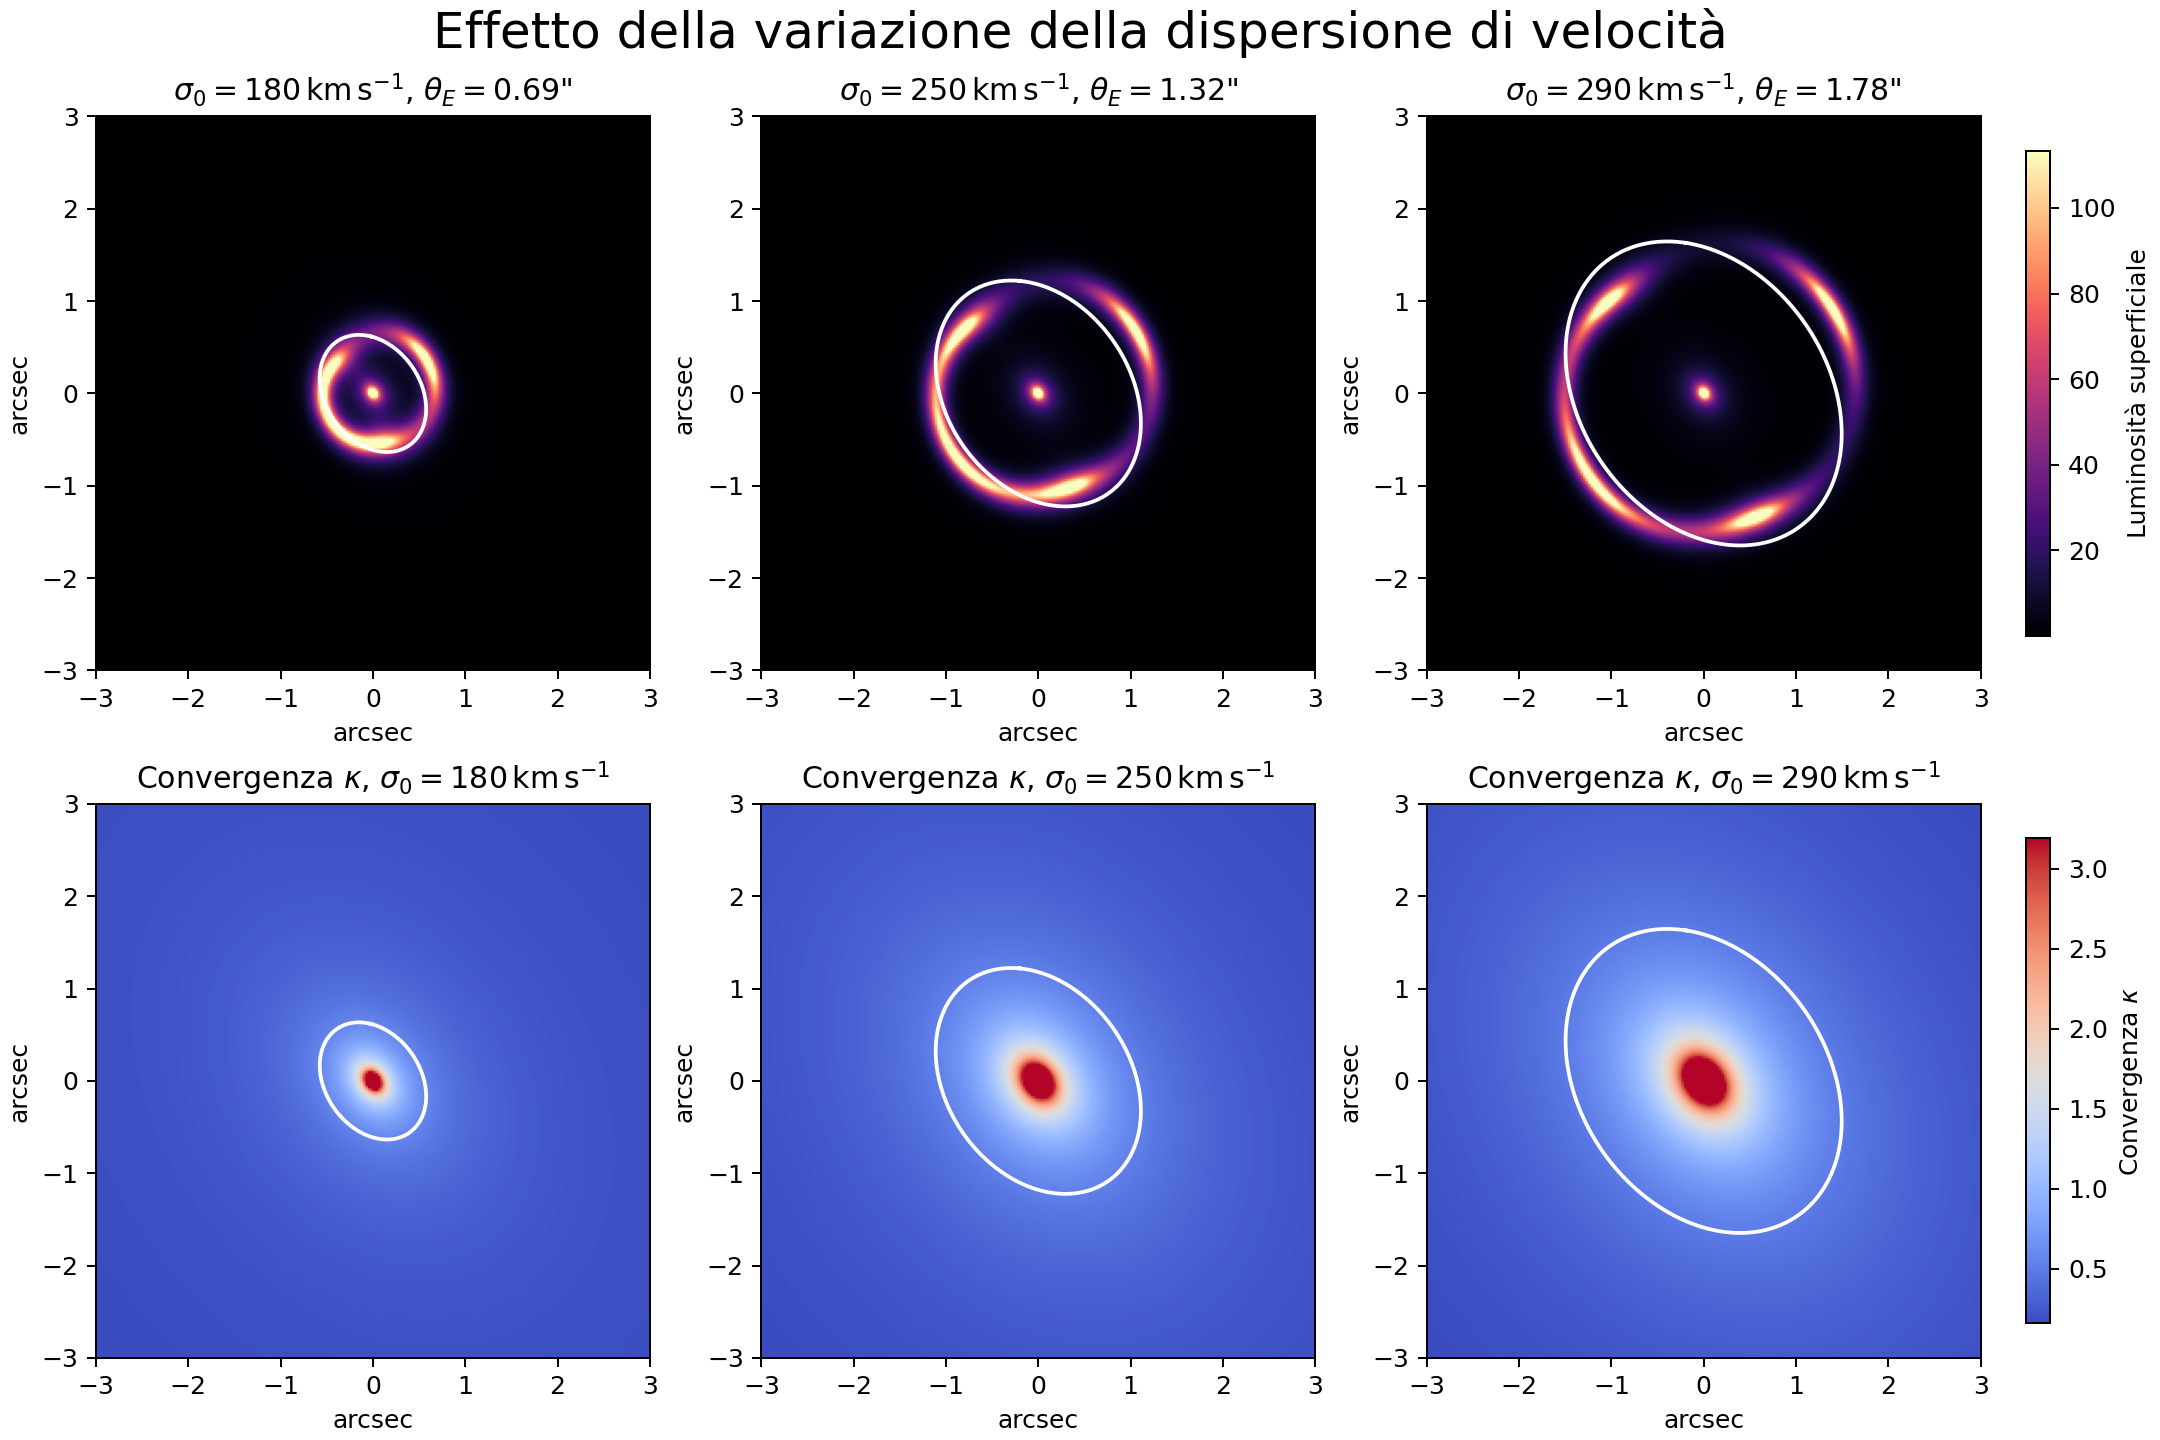
\includegraphics[width=\linewidth]{Immagini//4-Simulazioni/final_simulations_sigma0.png}
    \caption{Effetto dell'aumento della dispersione di velocità della galassia lente in un sistema di galaxy-galaxy lensing. Nei pannelli superiori sono riportate le immagini della sorgente lensata, a cui è stata sovrapposta la luce della lente, con relative dispersioni di velocità e raggi di Einstein. Nei pannelli inferiori, invece, sono riportate le relative mappe di convergenza. Su tutti i pannelli sono state disegnate le linee critiche (in bianco). Le immagini di una stessa riga sono riferite alla stessa scala, indicata dalla colorbar a destra, e sono dunque confrontabili fra loro.}
    \label{fig:sigma0_sim}
\end{figure}
Nei tre pannelli superiori si è riportata l'immagine composita della sorgente lensata e della luce della lente, a cui è stata sovrapposta la linea critica (in bianco). Si può notare che, a parità degli altri parametri, un aumento della dispersione di velocità ha come effetto l'aumento del raggio di Einstein, dato che aumentare $\sigma_0$ equivale ad aumentare la massa della lente. Ciò risulta coerente con quanto si era trovato nella formula \ref{eq:einstein_radius}: infatti, calcolando i rapporti tra le dispersioni di velocità massima e minima al quadrato si ha
\begin{equation}
    \Big(\frac{\sigma_{max}}{\sigma_{min}}\Big)^2 \simeq 2.60
\end{equation}
mentre calcolando il rapporto tra i relativi raggi di Einstein si trova
\begin{equation}
    \frac{\theta_{E,max}}{\theta_{E,min}}\simeq2.58
\end{equation}
da cui 
\begin{equation}
     \Big(\frac{\sigma_{max}}{\sigma_{min}}\Big)^2 \simeq \frac{\theta_{E,max}}{\theta_{E,min}}
\end{equation}
coerentemente con quanto atteso.
Tale aumento è chiaramente visibile anche nelle immagini, in quanto il raggio dell'anello di Einstein cresce guardando i pannelli da sinistra verso destra. 
Un altro dettaglio da cogliere è che galassie più massicce permettono una separazione angolare maggiore fra le immagini, rendendole distinguibili.
Nel primo pannello in alto a sinistra, infatti, tre delle quattro immagini previste teoricamente sono fuse in unico arco. Nel pannello centrale si iniziano a distinguere singolarmente e si può notare che due sono interne alla linea critica, mentre le altre due si trovano all'esterno. Nell'ultimo caso a destra le quattro immagini sono infine perfettamente distinte.

Nei tre pannelli inferiori sono riportate le mappe di convergenza relative alle immagini superiori, a cui sono state nuovamente sovrapposte le linee critiche. 
Considerando la formula \ref{eq:SIS_kappa}, la teoria prevede che, a parità di posizione angolare $\theta$ sul piano immagine, $\kappa$ aumenti linearmente con il raggio di Einstein; qualitativamente si osserva, infatti, che la regione a convergenza più alta si espande gradualmente al crescere di $\sigma_0$ (zona rossa).
La formula per le linee critiche tangenziali, ovvero quelle rappresentate in Figura \ref{fig:sigma0_sim}, per una lente generica, è 
\begin{equation}
     1-\kappa-\gamma =0
     \label{eq:tancl}
\end{equation}
dove si è omessa la dipendenza dei due parametri da $\theta$. Puntualmente, lo shear rimane costante nei tre casi, mentre $\kappa$ aumenta; per questo motivo, il luogo di punti  descritto da \ref{eq:tancl} si allontana progressivamente dal centro della galassia lente, ovvero si sposta a valori di $\theta$ maggiori, mantenendo però la stessa forma. Ciò è chiaramente visibile nelle ellissi di dimensioni crescenti sia nei pannelli superiori che in quelli inferiori. Si noti che l'ellitticità della linea critica è strettamente legata a quella della lente, dunque rimane invariata, così come la direzione dell'asse maggiore; ciò che cambia è unicamente la scala.
\subsection{Effetto del disallineamento rispetto alla linea di vista}
Come visto nella Sezione \ref{sez:Image formation}, a seconda della geometria del sistema cambiano sia la quantità di immagini prodotte che le loro proprietà. Per indagare questa fenomenologia, si è scelto di variare la posizione della sorgente mantenendo la lente fissa nell'origine. Si è dunque definita la lista 
\begin{lstlisting}
    positions = [(0.01, 0.03), (0.15, 0.1), (-0.15,0.05), (0.3, 0.3)]
\end{lstlisting}
in cui sono contenuti i valori dati in arcsec. Essi sono stati scelti in modo che la sorgente si trovasse nel primo caso quasi allineata alla lente, nel secondo vicino ad una cuspide della caustica, nel terzo vicino ad una \emph{fold} della caustica e nel quarto disallineata ed esterna alla caustica. In Figura \ref{fig:positions_sim} sono sintetizzati visivamente i risultati ottenuti. 
\begin{figure}[h]
    \centering
    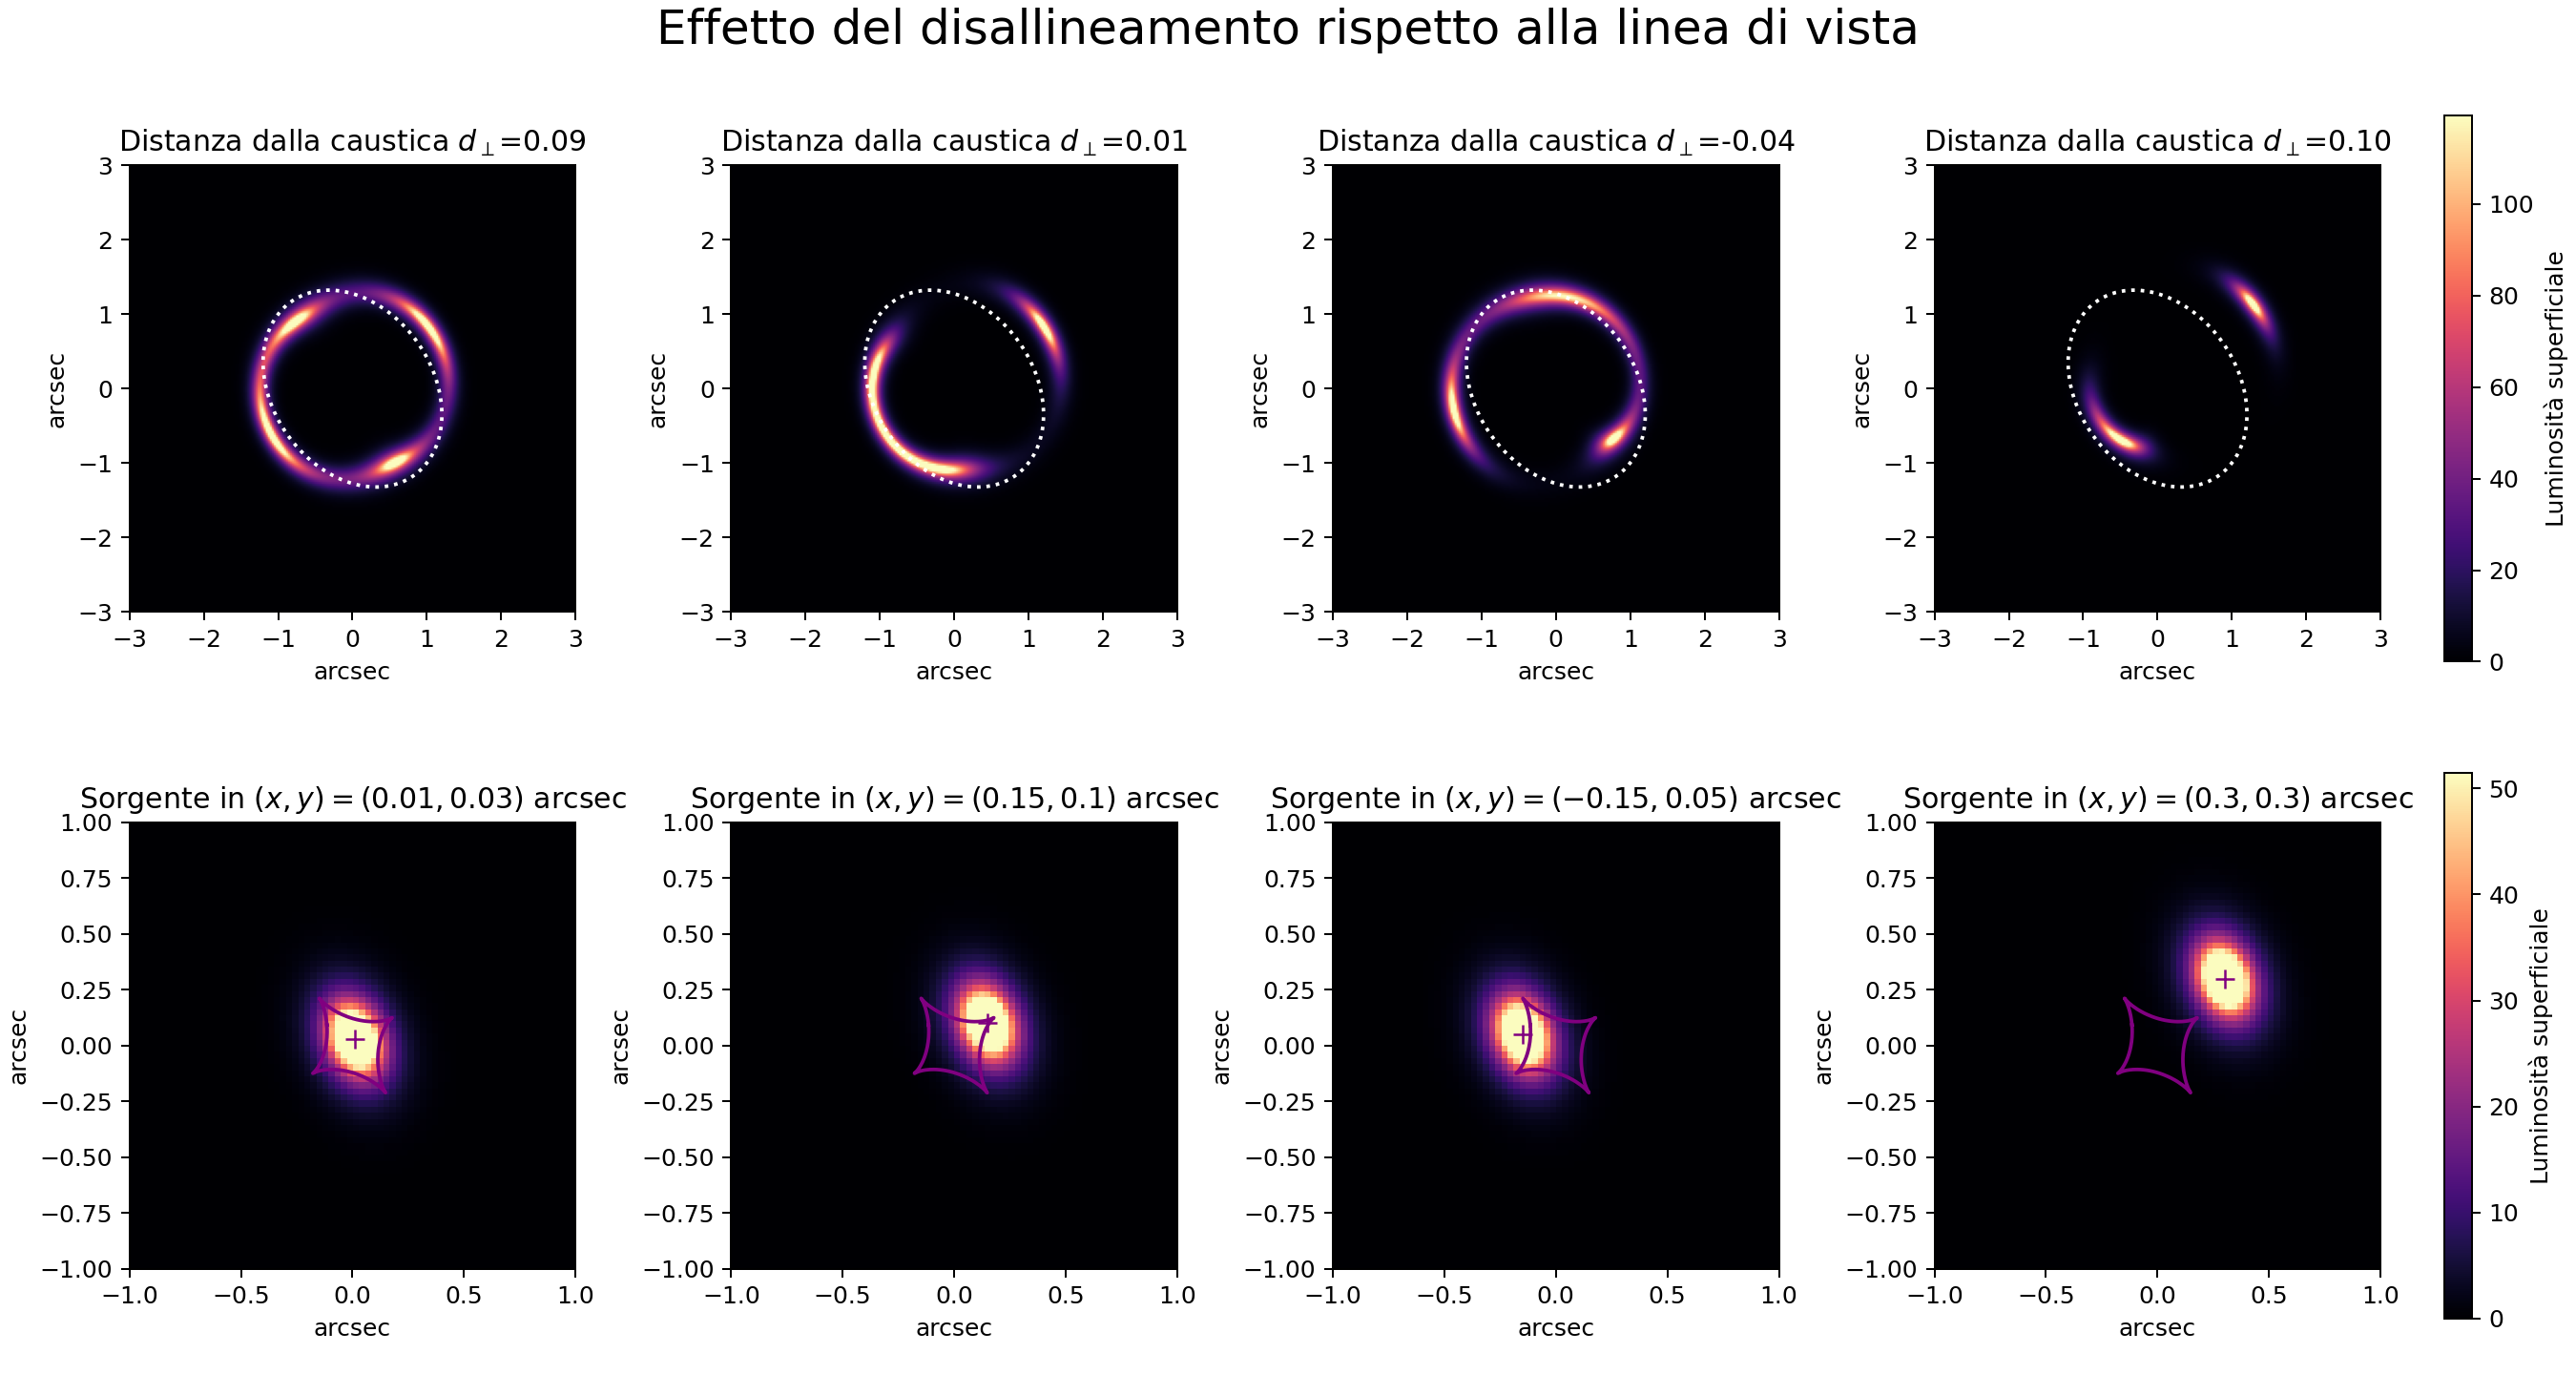
\includegraphics[width=\linewidth]{Immagini//4-Simulazioni/final_simulations_positions.png}
    \caption{Effetto del disallineamento rispetto alla linea di vista in un sistema di galaxy-galaxy lensing. Nei pannelli superiori sono riportate le immagini della sorgente lensata, con relativa distanza perpendicolare della sorgente dalla caustica. Ad esse sono state sovrapposte le linee critiche (in bianco, puntinate). Nei pannelli inferiori, invece, sono riportate le immagini della sorgente originaria, ingrandite su un campo visivo di 2.0" e con relativa posizione della sorgente. Ad esse sono state sovrapposte le caustiche (linee viola continue) e un marker indicante il centro della sorgente.  Le immagini di una stessa riga sono riferite alla stessa scala, indicata dalla colorbar a
destra, e sono dunque confrontabili fra loro. Le immagini di una stessa colonna, invece, essendo riferite a scale diverse, non lo sono.}
    \label{fig:positions_sim}
\end{figure}
Nei quattro pannelli superiori si è riportata l'immagine della sola sorgente lensata sul piano della lente, a cui è stata sovrapposta la linea critica (in bianco puntinato). Per etichettare le diverse configurazioni, è stata definita la quantità $d_\perp$, ovvero la distanza tra la sorgente e la caustica più vicina, proiettata sulla direzione normale alla curva in quel punto. Il segno indica da che lato della caustica si trova la sorgente: positivo all'interno, negativo all'esterno.
Nei quattro pannelli inferiori, invece, sono state riportate le immagini della sorgente originaria, su un campo visivo ridotto di 2.0", ovvero un terzo di quello totale. Ad esse sono state sovrapposte le caustiche e un marker per indicare la posizione del centro della sorgente (in viola). Nei titoli sono state riportate le coordinate della sorgente. 

Nella prima colonna, la sorgente è posta all'interno della caustica e vicina al suo centro, dove si trova la lente. Questo implica che sorgente e lente sono pressoché allineate rispetto alla linea di vista; la loro distanza euclidea è infatti pari a 
\begin{equation}
    d = \sqrt{0.01^2+0.03^2} \simeq 0.032\ \text{arcsec} 
\end{equation}
In questo caso, analogamente a quanto visto al variare di $\sigma_0$, si formano quattro immagini molto magnificate lungo l'anello di Einstein: due sono interne alla linea critica e sono di tipo II, mentre l'altra coppia è esterna ed è di tipo I. Sarebbe prevista anche un'immagine di tipo III centrale, ma essa risulta troppo debole per essere osservata. 

Nella seconda colonna, la sorgente è posta vicino ad una cuspide della caustica. La distanza euclidea tra la sorgente e la lente è pari a 
\begin{equation}
    d = \sqrt{0.15^2+0.1^2} \simeq 0.180\ \text{arcsec} 
\end{equation}
dunque esse risultano più lontane rispetto al caso precedente. La teoria, in questo caso, prevederebbe la formazione del cusp triplet, in cui sono presenti due immagini di tipo II ed una di tipo I; tuttavia, in questo caso le tre immagini non risultano angolarmente distinguibili, in quanto fuse in un unico arco gravitazionale molto brillante, interno alla linea critica. La quarta immagine, invece, si trova all'esterno e risulta molto meno magnificata; il flusso è  dominato dal tripletto.

Nella terza colonna, la sorgente è posta vicino ad una \emph{fold} della caustica. La distanza euclidea tra sorgente e lente è pari a 
\begin{equation}
    d = \sqrt{0.15^2+0.05^2} \simeq 0.158\ \text{arcsec} 
\end{equation}
L'attraversamento di una fold di una caustica prevede la nascita o la scomparsa di una coppia di immagini, una di tipo I e una di tipo II, a seconda del verso di attraversamento. Tale fenomeno è osservabile nel pannello superiore: si distingue una prima coppia di immagini, di cui una esterna e una interna alla linea critica, mentre la seconda, sovrapposta alla linea critica, è quella che sta scomparendo. 

Infine, nell'ultima colonna si è studiato un caso in cui la sorgente risulta esterna alla caustica e più distante rispetto alla linea di vista
\begin{equation}
    d = \sqrt{0.3^2+0.3^2} \simeq 0.424\ \text{arcsec} 
\end{equation}
In questo caso, si formano solo due immagini più compatte e meno magnificate, una interna alla linea critica (di tipo II) ed una esterna (di tipo I), coerentemente con quanto appena esposto. 

Da questa trattazione si osserva esattamente quanto discusso discorsivamente nel Capitolo \ref{cap:SGL}: all'aumentare del disallineamento del sistema, l'anello di Einstein si frantuma, dando luogo ad immagini multiple. L'attraversamento della caustica comporta un calo nel numero di immagini osservabili; delle quattro della prima colonna, infatti, nell'ultima ne sono rimaste solo due.  È inoltre interessante notare che, anche quando i moduli delle distanze dalla caustica o dalla linea di vista sono simili fra loro, la fenomenologia delle immagini può variare significativamente; questo è indice dell'importanza della topologia dello spazio e della curva, che non può essere riassunta in un unico valore. Tuttavia, si può notare che più basso è il valore di $d_\perp$, maggiore è la magnificazione delle immagini; la distanza dalla caustica incide dunque sulla brillantezza della configurazione.

\section{Introduzione di un perturbatore}
Finora si è analizzato come la morfologia delle immagini è influenzata da variazioni della configurazione geometrica del sistema e delle proprietà fisiche degli oggetti coinvolti. In questo paragrafo si introduce una sotto-struttura aggiuntiva, che produce perturbazioni locali al potenziale sulla base del proprio profilo di densità; in particolare vengono analizzati e confrontati il caso SIE ed il caso NFW. 
\subsection{Perturbatore modellato tramite profilo SIE}
Il primo modelling della struttura perturbatrice è avvenuto tramite un profilo analogo a quello della lente principale, ovvero il SIE (Eq. \ref{eq:rho_SIS} con cambio di variabile \ref{eq:ell_coordinate}). Analogamente a quanto fatto per il caso imperturbato, si sono studiati gli effetti di diversi valori della dispersione di velocità, o equivalentemente della massa dell'alone; in particolare si sono scelti i valori, espressi in km s$^{-1}$
\begin{lstlisting}
    sigma0_values_pert = [50.0, 70.0, 90.0]
\end{lstlisting}
che corrispondono approssimativamente a masse di, rispettivamente, $2\cdot 10^{8}\ M_\odot$, $8\cdot 10^{8}\ M_\odot$ e $2\cdot 10^{9}\ M_\odot$.
In Figura \ref{fig:SIE_sim} sono sintetizzati visivamente i risultati ottenuti; come riferimento, nella prima colonna è stato riportato il caso senza perturbatore. 
\begin{figure}
     \centering
     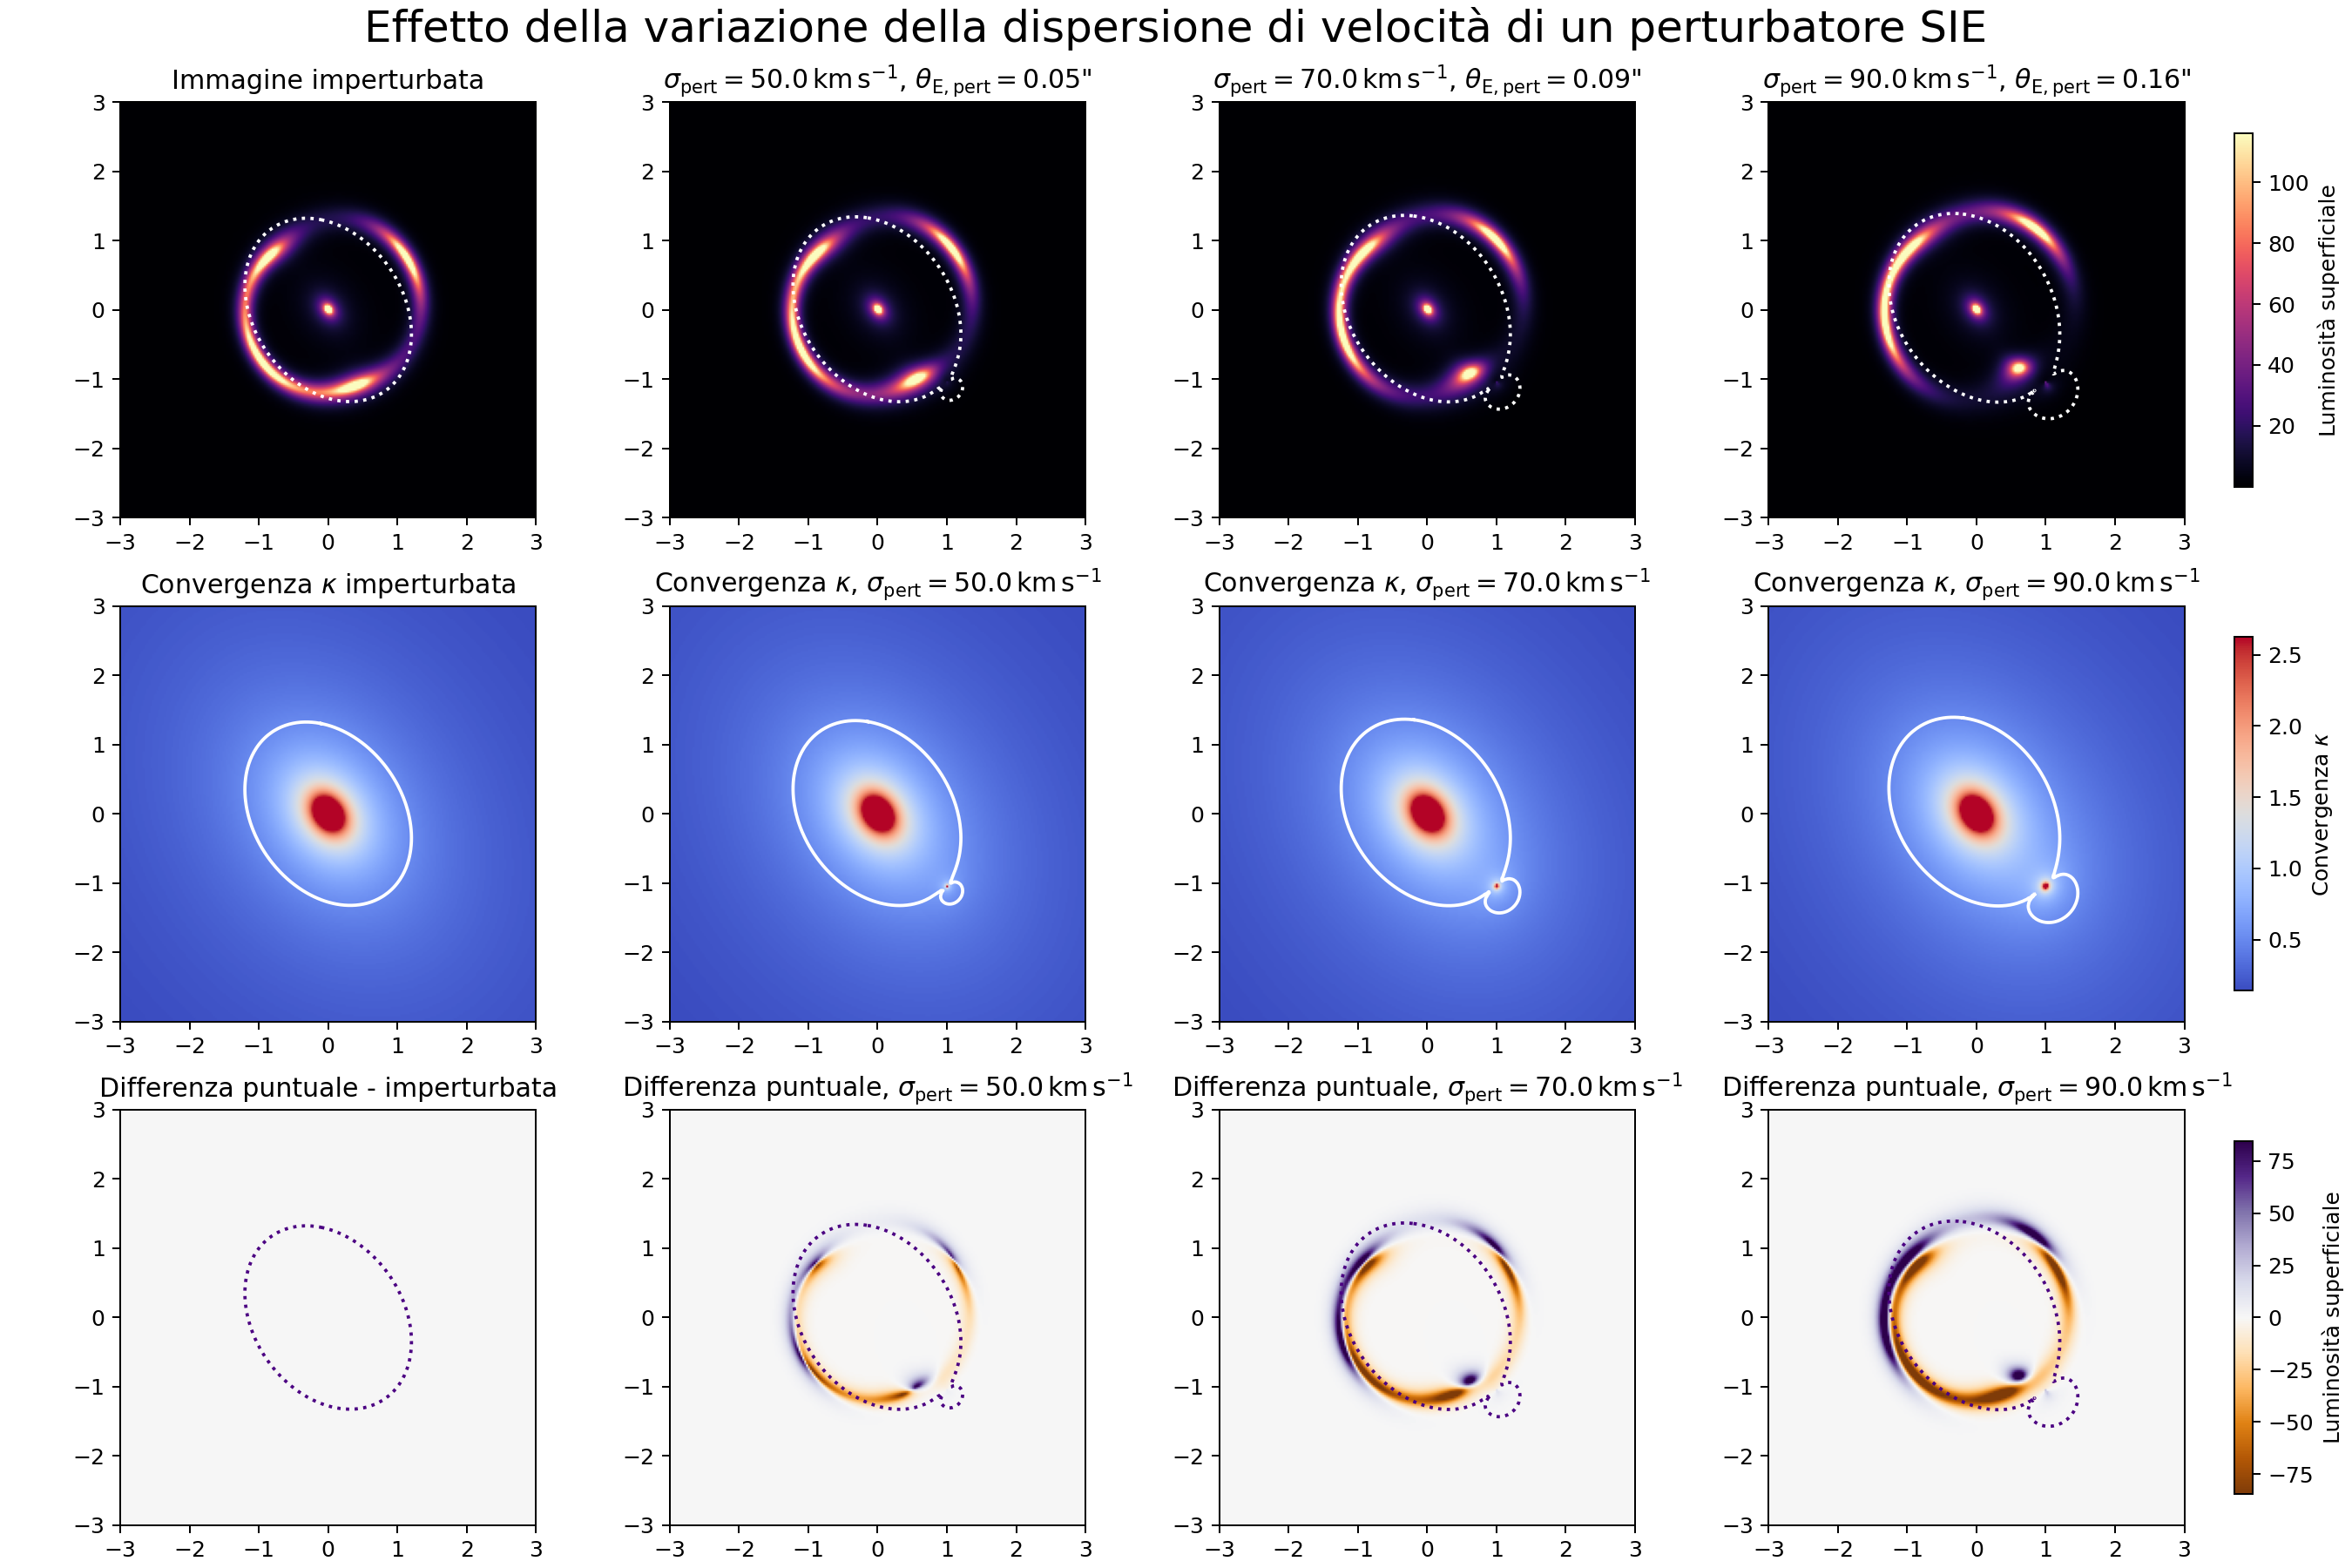
\includegraphics[width=\linewidth]{Immagini/4-Simulazioni/final_simulations_SIE.png}
     \caption{Effetto dell'aggiunta di un perturbatore con profilo SIE di massa crescente in un sistema di galaxy-galaxy lensing. Nei pannelli superiori sono riportate le immagini della sorgente lensata, a cui è stata sovrapposta la luce della lente, con relative dispersioni di velocità e raggi di Einstein del perturbatore. Nei pannelli intermedi sono riportate le relative mappe di convergenza.
     Infine, nei pannelli inferiori sono riportate le differenze tra l'immagine perturbata e quella imperturbata. Nella prima colonna sono riportati in tutti i casi i riferimenti imperturbati. Su tutti i pannelli sono state disegnate le linee critiche (punteggiate sopra, linee continue nella riga intermedia, in viola sotto). Le immagini di una stessa riga sono riferite alla stessa scala, indicata dalla colorbar a
     destra, e sono dunque confrontabili fra loro.}
     \label{fig:SIE_sim}
 \end{figure}
Nei quattro pannelli superiori sono rappresentate le immagini composite della sorgente lensata e della luce della lente, a cui sono state sovrapposte le relative linee critiche (in bianco, puntinate). Analogamente a quanto accade per la lente principale, un aumento della dispersione di velocità ha come effetto l'aumento del raggio di Einstein del perturbatore, coerentemente con la relazione precedente. Calcolando il rapporto delle dispersioni massima e minima al quadrato si ha
\begin{equation}
    \Big(\frac{\sigma_{max,\ pert}}{\sigma_{min,\ pert}}\Big)^2 = 3.24
\end{equation}
mentre calcolando il rapporto dei raggi di Einstein si trova
\begin{equation}
    \frac{\theta_{E,max}}{\theta_{E,min}}=3.20
\end{equation}
da cui nuovamente 
\begin{equation}
    \Big(\frac{\sigma_{max,\ pert}}{\sigma_{min,\ pert}}\Big)^2 \simeq  \frac{\theta_{E,max}}{\theta_{E,min}}
\end{equation}
Inoltre, con l'intensificarsi della perturbazione, l'immagine della sorgente in basso a destra diventa progressivamente meno estesa ed intensa, e aumenta la sua separazione angolare rispetto all'arco adiacente. Nell'ultimo pannello, si può anche notare la formazione di una nuova immagine poco brillante in prossimità della sotto-struttura. Tali effetti sono coerenti con le perturbazioni alla brillanza superficiale discusse nella Sezione \ref{sez:I_perturbations}.

Nei quattro pannelli intermedi, invece, sono riportate le mappe di convergenza relative alle immagini superiori, a cui sono state nuovamente sovrapposte le linee critiche.
In analogia con quanto già visto, la regione a convergenza più alta in corrispondenza del perturbatore (puntino rosso in basso a destra) si espande gradualmente al crescere di $\sigma_{pert}$. Con essa si estende anche la linea critica del perturbatore, di forma ellittica; di conseguenza, la linea critica complessiva viene deformata localmente, fondendo fra loro due ellissi di ellitticità differenti e disposte in maniera diversa nello spazio. 

Infine, nella riga inferiore sono riportate le differenze puntuali tra l'immagine in cui è presente il perturbatore e il caso imperturbato. Nel primo pannello si osserva uno sfondo uniformemente bianco, in quanto l'immagine imperturbata è stata sottratta a se stessa. Nei pannelli successivi si vedono gradualmente comparire i residui, che si intensificano con l'aumento di $\sigma_{pert}$; le tracce in arancione identificano un calo nella brillanza superficiale, e indicano dunque la posizione delle immagini in assenza del sotto-alone. Le tracce in viola, invece, mostrano un aumento della brillanza superficiale a seguito della perturbazione. Cali e aumenti risultano essere sempre adiacenti tra loro e situati in prossimità dell'anello; ciò indica che l'aggiunta della sotto-struttura causa una traslazione e un rimodellamento delle immagini, dovuti ad un cambiamento nel campo gravitazionale, e di conseguenza nell'angolo di deflessione.

Per quantificare la firma gravitazionale lasciata dal perturbatore nel modello, visualizzata finora solo in maniera puntuale, si è definita la grandezza 
\begin{lstlisting}
    flux_ratio = (
    source_with_second.image.sum()
    - source.image.sum()
    ) / source.image.sum()
\end{lstlisting}
ovvero la differenza fra il flusso totale dell'immagine con perturbatore e quella imperturbata, normalizzata rispetto al flusso totale imperturbato. 
In Figura \ref{fig:SIE_graph_sim} è riportato un grafico che mostra la \texttt{flux\_ratio} al variare della dispersione di velocità, per $\sigma_{pert}$ che passa da 0 a 90 km s$^{-1}$ ad intervalli di 10.
 \begin{figure}[h]
     \centering
     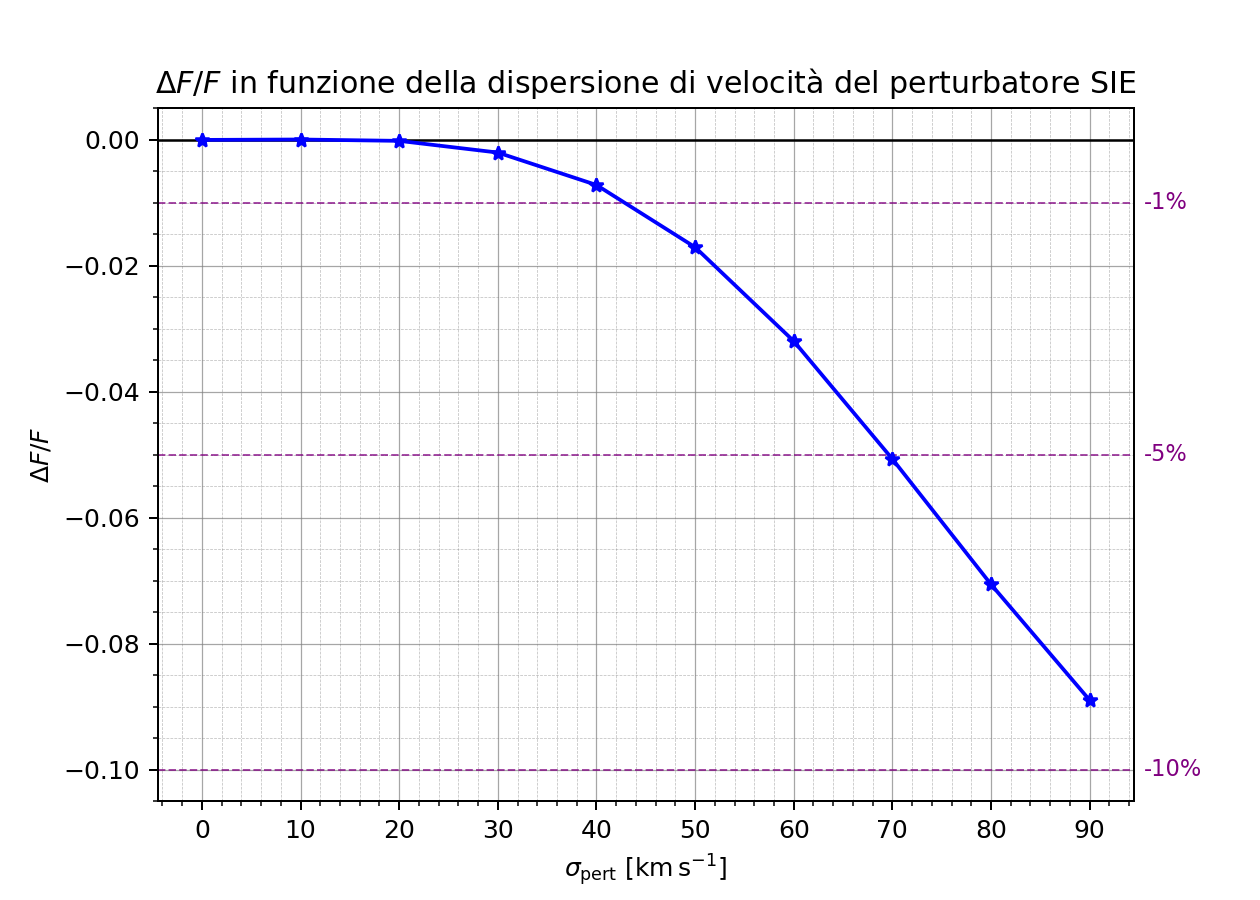
\includegraphics[width=0.7\linewidth]{Immagini/4-Simulazioni/final_simulations_SIE_graph.png}
     \caption{Differenza fra il flusso totale dell'immagine con perturbatore e quella imperturbata, normalizzata rispetto al flusso totale imperturbato, al variare della dispersione di velocità del perturbatore SIE. In blu sono rappresentati i valori simulati, connessi da una linea per mostrarne l'andamento. In viola invece, sono rappresentate le soglie per una diminuzione, dall'alto verso il basso, dell'1\%, del 5\% e del 10\%.}
     \label{fig:SIE_graph_sim}
 \end{figure}
 Da esso può essere confermato quantitativamente quanto era già stato intuito qualitativamente: nel complesso, si ha una progressiva diminuzione di flusso all'aumentare della dispersione di velocità del satellite. In particolare, per $\sigma_{pert}= 50.0$ km s$^{-1}$ si ha $\frac{\Delta F}{F}=-1.7 \%$, per $\sigma_{pert}= 70.0$ km s$^{-1}$ si ha $\frac{\Delta F}{F}=-5.1 \%$ e infine per $\sigma_{pert}= 90.0$ km s$^{-1}$ si ha $\frac{\Delta F}{F}=-8.9\%$.
 Poiché il profilo SIE ha un andamento $1/r^2$ per $r \to 0$, le sotto-strutture modellate risultano molto compatte, e sono lenti molto efficienti; infatti, anche per dispersioni di velocità relativamente basse (ad esempio 40 km s$^{-1}$) si ottengono già anomalie di flusso dell'ordine del percento. Ciò rende gli effetti degli aloni più semplici da rilevare rispetto a profili che, a parità di massa, risultano più diffusi, come emergerà chiaramente nella trattazione del perturbatore NFW. 

\subsection{Perturbatore modellato tramite profilo NFW}
Come visto nel Capitolo \ref{cap:cosmologia}, un profilo di densità migliore per descrivere nello specifico le sotto-strutture di materia oscura è il profilo NFW (Eq. \ref{eq:NFW}). Se per il profilo SIE il parametro caratteristico è la dispersione di velocità, per il profilo NFW le due grandezze che determinano la forma della curva sono la massa $M_{pert}$ e la concentrazione $c$. Nell'analisi di questa tesi, la concentrazione viene mantenuta costante, mentre viene variata la massa dell'alone; in particolare, sulla base degli articoli presentati e citati nelle rilevazioni individuali del Capitolo \ref{cap:SGL+DM}, si sono scelti 
\begin{lstlisting}
    mass_values = [5.0e8, 7.0e9, 1.0e11]
\end{lstlisting}
espressi in unità di masse solari $M_\odot$.
In Figura \ref{fig:NFW_sim} sono sintetizzati visivamente i risultati ottenuti; anche in questo caso, nella prima colonna è stato riportato il caso senza perturbatore come riferimento. 
\begin{figure}
    \centering
    
\includegraphics[width=\linewidth]{Immagini/4-Simulazioni/final_simulations_NFW.png}
    \caption{Effetto dell'aggiunta di un perturbatore con profilo NFW di massa crescente in un sistema di galaxy-galaxy lensing. Nei pannelli superiori sono riportate le immagini della sorgente lensata, a cui è stata sovrapposta la luce della lente, con relative masse e raggi di scala del perturbatore. Nei pannelli intermedi sono riportate le relative mappe di convergenza. 
    Infine, nei pannelli inferiori sono riportate le differenze tra l'immagine perturbata e quella imperturbata. Nella prima colonna sono riportati in tutti i casi i riferimenti imperturbati. Su tutti i pannelli sono state disegnate le linee critiche (punteggiate sopra, linee continue nella riga intermedia, in viola sotto). Le immagini di una stessa riga sono riferite alla stessa scala, indicata dalla colorbar a destra, e sono dunque confrontabili fra loro.}
    \label{fig:NFW_sim}
\end{figure}

Nei quattro pannelli superiori sono rappresentate le immagini composite della sorgente lensata e della luce della lente, a cui sono state sovrapposte le relative linee critiche (in bianco, puntinate). Nel caso del profilo NFW è importante ricordare che esso decade a grandi r come $1/r^3$. Di conseguenza, le masse nominali riportate sopra corrispondono all'integrazione della densità di massa da zero all'infinito, e possono essere sensibilmente maggiori rispetto alla massa proiettata entro l'area effettivamente rilevante per il lensing. Inoltre, per $r \to 0$ il profilo NFW ha un andamento più dolce del SIE, in quanto cresce come $1/r$. Di conseguenza, anche a parità di massa proiettata, un alone NFW è meno concentrato rispetto ad un SIE: la lente gravitazionale che ne risulta è meno efficace, e gli effetti osservabili sono meno evidenti. 

Ciò si manifesta anche a livello simulativo. Infatti, osservando i pannelli superiori, la presenza di un perturbatore di massa dell'ordine di $10^8$ o $10^9$ masse solari non presenta perturbazioni di brillanza superficiali evidenti, come invece accadeva nel caso SIE. Solo nell'ultimo caso, per $M_{pert}=1 \cdot 10^{11}\ M_\odot$, dove l'alone sarebbe abbastanza massiccio da presentare materia luminosa al proprio interno, si nota una deformazione delle immagini. In particolare, quella in basso a destra diminuisce la propria estensione ed aumenta la propria separazione angolare rispetto alle altre, che invece si avvicinano fra loro e tendono a fondersi in un unico arco gravitazionale. 
Un'altra differenza rispetto al profilo SIE è proprio questa: esso risulta molto concentrato, quindi le anomalie più evidenti si riscontrano solo nell'immagine in prossimità del perturbatore. Il profilo NFW, invece, sebbene causi localmente deformazioni meno evidenti, mostra anomalie alla brillanza superficiale diffuse tra tutte le immagini. Ciò lo rende nettamente più difficile da distinguere dagli effetti geometrici e fisici del sistema. 

La minor concentrazione degli aloni si riflette anche nelle mappe di convergenza riportate nei pannelli intermedi. Infatti, la deformazione delle linee critiche nei primi due casi perturbati è appena percettibile, e non si osservano i picchi di convergenza evidenti del caso ellittico; solo nell'ultimo pannello si manifestano fenomenologie simili al caso precedente, e si può notare che la curva critica si deforma in maniera simile a quanto accadeva nel SIE.

Una particolarità del profilo NFW rispetto al SIE è che, anche se la firma di una sotto-struttura non è evidente dalle immagini spettrometriche, essa può essere rilevata dai residui. Ciò è chiaro anche osservando anche la riga inferiore della Figura \ref{fig:NFW_sim}: confrontando i vari casi con quello imperturbato a sinistra, per il secondo pannello la differenza è appena percepibile, ma già ad una massa di $M_{pert}=7 \cdot 10^{9}\ M_\odot$ la firma del sotto-alone è chiaramente visibile; nell'ultimo caso si hanno poi effetti macroscopici evidenti. È dunque chiaro che l'entità della perturbazione cresce all'aumentare della massa della sotto-struttura. Anche in questo caso, inoltre, le zone arancioni corrispondenti ai cali e quelle viola corrispondenti agli aumenti della luminosità superficiale risultano sempre accoppiate fra loro e poste in prossimità degli archi, indicando una traslazione e un rimodellamento delle immagini causati dal cambiamento nel potenziale gravitazionale del sistema. 

Successivamente, si è adottata la \texttt{flux\_ratio} per quantificare la firma gravitazionale lasciata dal perturbatore nel modello; in Figura \ref{fig:NFW_graph_sim} è riportato il suo andamento al variare della massa dell'alone. 
\begin{figure}
    \centering
    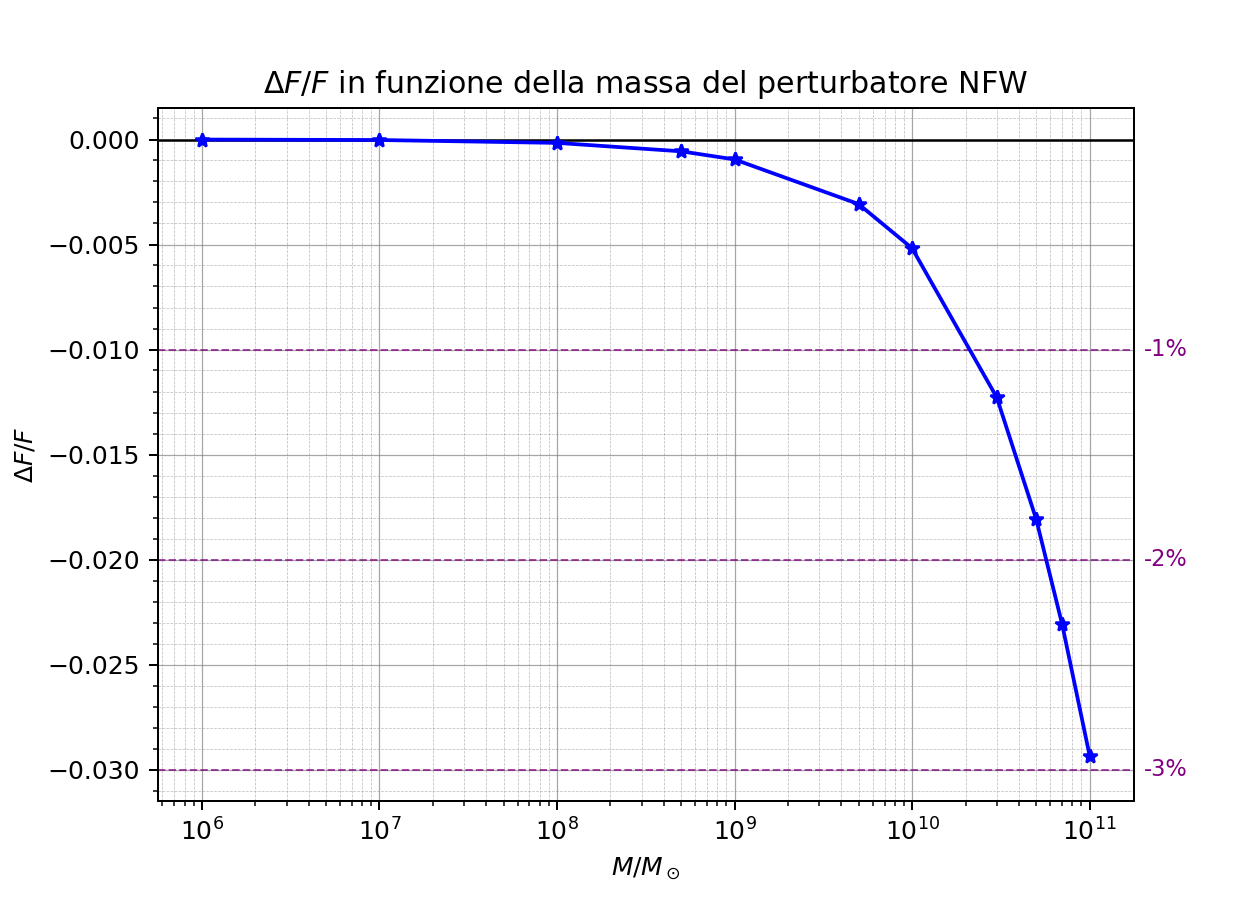
\includegraphics[width=0.7\linewidth]{Immagini/4-Simulazioni/final_simulations_NFW_graph.png}
    \caption{Differenza fra il flusso totale dell'immagine con perturbatore e quella imperturbata, normalizzata rispetto al flusso totale imperturbato, al variare della massa del perturbatore NFW. In blu sono rappresentati i valori simulati, connessi da una linea per mostrarne l'andamento. In viola invece, sono rappresentate le soglie per una diminuzione, dall'alto verso il basso, dell'1\%, del 2\% e del 3\%. L'asse delle masse è stato visualizzato in scala logaritmica.}
    \label{fig:NFW_graph_sim}
\end{figure}

Si nota nuovamente una progressiva diminuzione di flusso all'aumentare della massa della sotto-struttura; in particolare, per $M_{pert}=5 \cdot 10^{8}\ M_\odot$ si ha $\frac{\Delta F}{F}=-0.06\%$, per $M_{pert}=7 \cdot 10^{9}\ M_\odot$ si ha $\frac{\Delta F}{F}=-0.39\%$ e infine per $M_{pert}=1 \cdot 10^{11}\ M_\odot$ si ha $\frac{\Delta F}{F}=-2.93\%$. Tali valori sono stati calcolati all'interno del codice; per disegnare il grafico si è utilizzato il campionamento più grossolano 
\begin{lstlisting}
    mass_values_graph = [1.0e6, 1.0e7, 1.0e8, 5.0e8, 1.0e9, 5.0e9, 1.0e10, 3.0e10, 5.0e10, 7.0e10, 1.0e11]
\end{lstlisting}
Osservando il grafico ed i valori riportati nel testo è evidente che, poiché le sotto-strutture NFW più piccole causano anomalie di flusso inferiori al punto percentuale, rilevarle può diventare complesso e richiedere un'alta risoluzione strumentale. 
Tuttavia, come visto ampiamente nei capitoli precedenti, sono proprio i sotto-aloni meno massivi a porre i vincoli più importanti sulla natura della materia oscura, in quanto è alle masse più basse che si hanno le maggiori divergenze tra i modelli teorici.

In conclusione, quanto presentato in questo capitolo conferma come il lensing gravitazionale sia uno strumento particolarmente sensibile per lo studio della materia oscura. Tuttavia, la presente trattazione non tiene conto di fattori fondamentali nelle rilevazioni reali, quali il rumore strumentale, la risoluzione del telescopio usato o l'influenza che la materia barionica circostante può avere sul sistema. Le simulazioni presentate permettono dunque di comprendere la morfologia generale delle immagini e costituiscono un utile banco di prova per studiare le numerose condizioni geometriche, fisiche e strumentali che caratterizzano un sistema osservativo; esse però non sono da considerare confrontabili con rilevazioni reali, le quali presentano tutte le complicazioni già discusse nei capitoli precedenti.

